

%template setup, made it adhere to UWA standards
\documentclass[12pt, a4paper]{article}
\usepackage{graphicx}
\usepackage{amsmath}
\setlength{\oddsidemargin}{0.5cm}
\setlength{\evensidemargin}{0.5cm}
\setlength{\topmargin}{-1.6cm}
\setlength{\leftmargin}{0.5cm}
\setlength{\rightmargin}{0.5cm}
\setlength{\textheight}{24.00cm} 
\setlength{\textwidth}{15.00cm}
\parindent 0pt
\parskip 5pt
\pagestyle{plain}


%meta info
\title{Beyond the Thermodynamic Hypothesis}
\author{Max Ward \\
School of Computer Science \& Software Engineering \\
The University of Western Australia}
%let the date get auto generated

%author list formatter. not really needed here, but always nice to have
\newcommand{\namelistlabel}[1]{\mbox{#1}\hfil}
\newenvironment{namelist}[1]{%1
\begin{list}{}
    {
        \let\makelabel\namelistlabel
        \settowidth{\labelwidth}{#1}
        \setlength{\leftmargin}{1.1\labelwidth}
    }
  }{%1
\end{list}}



%-------------------------------------------------------------------------

\begin{document}


%title first!
\maketitle

\begin{abstract}
The algorithmic prediction of RNA molecules dates back to the late 1970s. Despite the field's age, little progress has been made. There are two core approaches for in silico RNA folding: ad-hoc dynamic programming algorithms, and stochastic context free grammar parsing methods. Both converge on the same accuracy upper limit, despite often using wildly different scoring schemes. In this report I outline these core algorithmic approaches for folding RNA. Furthermore, I highlight the lack of progress in prediction accuracy. Finally, I attempt to explain why the predictive power of these algorithms is stunted, and suggest a direction for future research.
\end{abstract}


{\bf Keywords:} Ribonucleic acid, structure, prediction, thermodynamic hypothesis.

{\bf CR Classification:} J.3 Biology and genetics.

\clearpage

\tableofcontents
\listoffigures
\clearpage

\section{Introduction}
This report outlines the algorithmic prediction of Ribonucleic Acid (RNA) structures. An overview of the essential techniques is given. In particular, the lack of significant progress is stressed, and possible explanations are explored. However, we must first understand what RNA is, and how they fold. RNA molecules fold much like paper aeroplanes. To understand this, the reader must also understand the chemistry of RNA, which is straightforward, and for which I shall now describe a working model.

\section{RNA and Aeroplanes} 
As the name implies, RNA is chemically similar to Deoxyribonucleic Acid (DNA). However, unlike DNA, RNA is single stranded. This means that it is made of a single sequence of connected nucleotides. These nucleotides are like links in a chain. Each such nucleotide is attached to its direct neighbours in the sequence. Much like an actual chain, a complete RNA sequence is flexible, and can move about freely. While the nucleotides I have mentioned are chemically ingenious, we need not know the details. All that need be said here is that there are four types: Adenine (often abbreviated to A), Guanine (G), Cytosine (C), and Uracil (U). Adenine readily forms chemical bonds with Uracil, and vice-versa. Similarly, Guanine and Cytosine have a propensity to bond. Additionally, Guanine and Uracil sometimes form weak bonds. In the parlance of RNA research, these types of bonds are called `A-U', `G-C', and `G-U' respectively.


So what about the paper aeroplanes? When constructing such a machine, one starts with a blank sheet of paper, and folds it repeatedly upon itself. This is precisely what happens when RNA molecules form bonds. Say a G and C nucleotide began forming a chemical bond. This would cause the entire chain to fold on itself as the G and C nucleotides come into close proximity. After the bond has formed, we are left with a loop containing the nucleotides that were between the G and the C in our theoretical RNA (see Figure \ref{fig:RNAssBasic}). The folding process may then repeat itself for nucleotides that are contained inside this loop region. Hence we say that the bonds of RNA molecules are nested (see Figure \ref{fig:RNAss} for a visual example). Folds form within folds; the structure of RNA is recursive. To clarify these concepts, let us recapitulate the paper aeroplane analogy. Paper aeroplanes are made from finite, two dimensional rectangles that fold repeatedly in three dimensions. In contrast, RNA molecules are finite, one dimensional line segments that fold repeatedly in two dimensions. More detail can be found in ``How RNA Fold'' which was published in the \emph{Journal of Molecular Biology} \cite{tinoco1999rna}.

\begin{figure}
\begin{center}
%the image is quite large, needs to be scaled dwon
\scalebox{0.7}{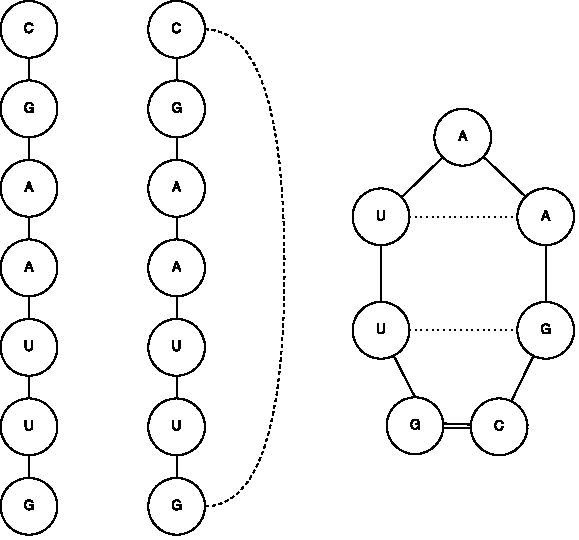
\includegraphics{RNAssBasic}}
\end{center}
\caption{A simple example of how a RNA sequence might fold. Dotted lines represent potential bonds between nucleotides, double lines represent actual bonds. The progression of folding follows from left to right.}
\label{fig:RNAssBasic}
\end{figure}


\subsection{The Importance of RNA}

RNA molecules fold into interesting structures, but why do they matter? RNA is actually a biologically active molecule. Recent research has found myriad functions for RNA. For example, RNA can alter the regulation of genes, acts as a catalyst for mRNA splicing, and is involved in peptide bond formation
\cite{xu2012statistical}. It is axiomatic that chemical structure is tantamount to biological function, and RNA is no exception. For this reason, there has and continues to be an intense
interest in predicting the structure of RNA
molecules in silico. Furthermore, it will allow the detection and classification of unknown RNAs, and assist the design of new RNA based drugs \cite{condon2003problems}. The structure of RNA
is also highly conserved during evolution, indicating its importance \cite{hofacker2008rna}.

I endeavour to give the reader a brisk but incisive review of RNA secondary structure prediction algorithms in this report. For the sake of succinctness, my focus shall be methods able to predict RNA structures ex nihilo---that is, with no information other than the RNA sequence itself. Additionally, I have omitted algorithms capable of predicting structures called pseudoknots. This is because such structures are uncommon, and because prediction of RNA structures with pseudoknots is an NP-complete problem \cite{lyngso2000rna}. The reader should also note that the kinds of structures I have described here are called `secondary structures'. The primary structure of RNA is simply the chain of nucleotides. Thus, as I have explained, the secondary structure of RNA is its two dimensional shape after folding. This shape is what is computed by `secondary structure prediction' algorithms. The most popular secondary structure prediction algorithms are those utilizing dynamic programming.

\begin{figure}
\begin{center}
%the image is quite large, needs to be scaled dwon
\scalebox{0.17}{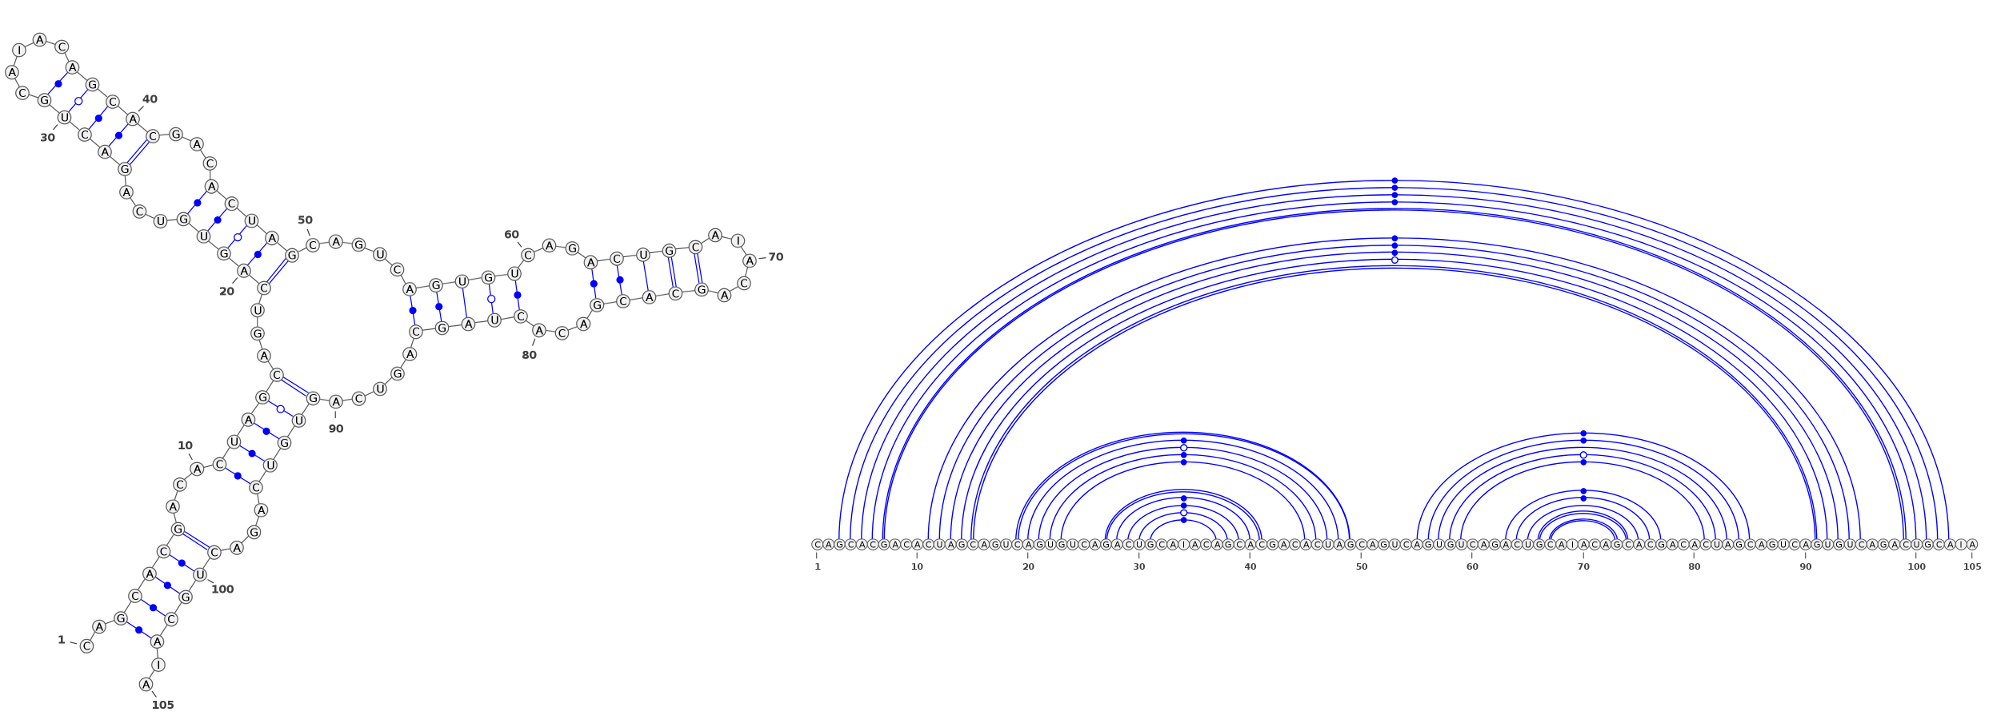
\includegraphics{RNAss}}
\end{center}
\caption{How a real RNA might fold. Depicted on the left is the final folded state of a sample RNA. Blue lines represent bonds between nucleotides. Depicted on the right is the same RNA structure organized into an arc diagram. In an arc diagram the RNA nucleotide chain is laid out lengthwise; blue arcs correspond to bonds in the diagram on the left. The arc diagram is included here to illustrate how bonds are contained recursively within other bonds.}
\label{fig:RNAss}
\end{figure}

\section{Dynamic Programming}
\subsection{The Nussinov Algorithm}
According to the `Thermodynamic Hypothesis', biologically active molecules should form structures that have minimum free energy and thus maximum stability \cite{anfinsen1973principles}. For RNA molecules, counting bonds is a crude but nonetheless accurate measure of energetic stability, as every bond increases the
stability of a structure \cite{nussinov1978algorithms}. In the late 1970s, when the first large RNA molecules
were being successfully sequenced, Nussinov et al. \cite{nussinov1978algorithms} introduced an algorithm to find a single structure with maximal number of bonds using dynamic programming. This is possible only with the restriction that all bonding pairs are nested. Fortunately this is true of RNA secondary structures as they form by repeated folding. The nested nature of bonds is elucidated by Figure \ref{fig:RNAss}.

Shortly after this, Nussinov \& Jacobson \cite{nussinov1980fast} introduced
a refined version of the same algorithm. They also tested it against experimentally verified RNA secondary structures. They had mixed success; transfer RNAs
(tRNAs) were conspicuous in their difference from predicted structures. They extended the algorithm to accommodate a more advanced energy model. Instead of weighting each bond equally, bonds are weighted
according to the proportion they are expected to contribute to the molecule's
stability. When considering the value of a bond, it might be given greater
weight if it adds to the formation of a stem (a stabilizing structure), or
given lower weight if it forms an internal loop or bulge, as these generally
destabilize RNA molecules. Unfortunately it is hard to find good values for
such weights, and determining which substructure a bond contributes to requires
backtracking. This caused the modified algorithm of Nussinov \& Jacobson to run slower than the original algorithm.

\subsection{The Zuker Algorithm}
Soon after the work of Nussinov \& Jacobson, Zuker \& Stiegler \cite{zuker1981optimal}
described an altered version of the same algorithm which, instead of maximising
bond weights, minimized free energy. The lower free energy a molecule has, the more stable it is. This was done
by introducing a number of thermodynamic rules for canonical substructures like hairpin loops, internal bulges, multiloops (also called bifurcation loops), unbonded bases, and stacked base pairs. For examples of these structures, refer to Figure \ref{fig:zuk_struct}. The Zuker algorithm is similar to the Nussinov algorithm,
but requires another mutually recursive dynamic programming recurrence to inject a relatively comprehensive scoring scheme. The thermodynamic scoring system is borrowed from the work of Studnicka et al. \cite{studnicka1978computer} who presented a
complex but theoretically similar algorithm, albeit having
much worse asymptotic and implementation complexity. 

\begin{figure}
\begin{center}
\scalebox{0.27}{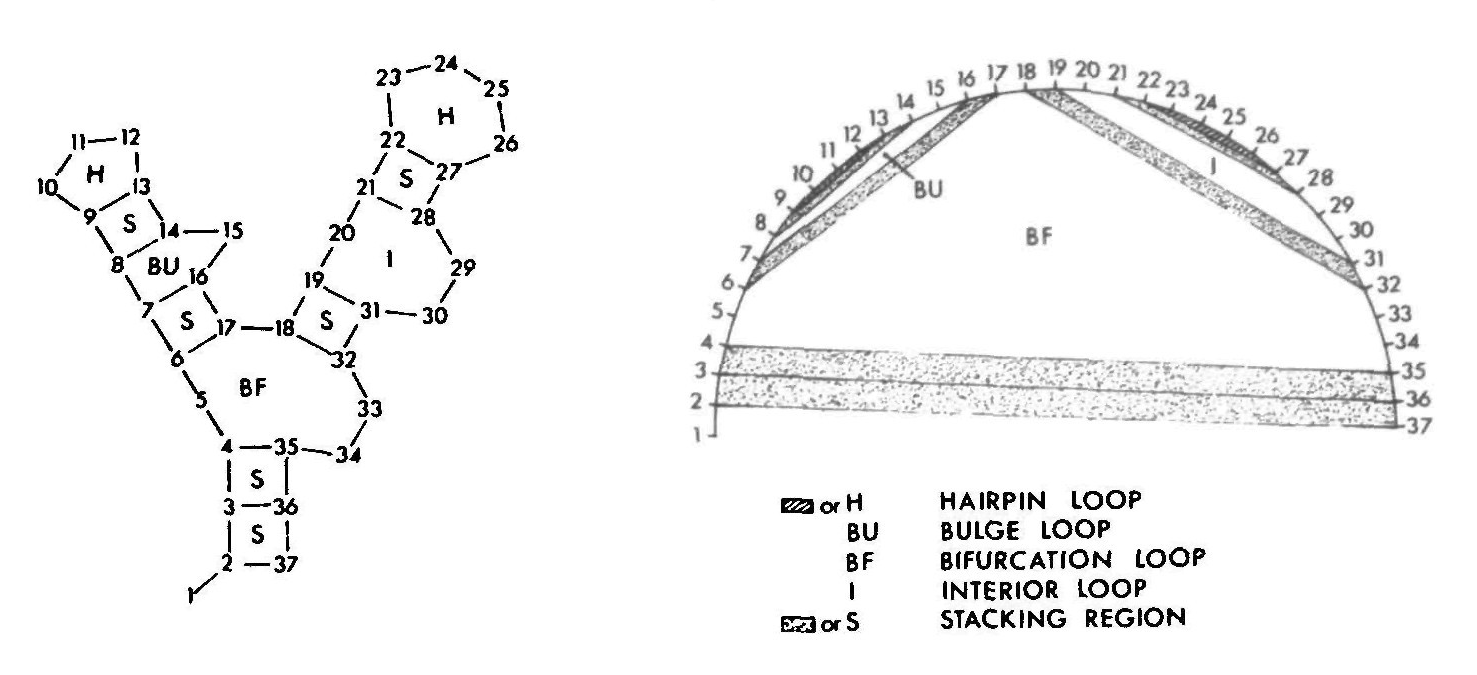
\includegraphics{figure4}}
\end{center}
\caption{Diagram of substructures used in the Zuker algorithm. On the left is a diagram of a RNA secondary structure. On the right is the same structure laid out on a semi-circle. Bonds are represented as lines crossing the semi-circle. Taken from original
publication \cite{zuker1981optimal}.}
\label{fig:zuk_struct}
\end{figure}


The algorithm of Zuker \& Stiegler \cite{zuker1981optimal} has some problems, however. Because there exist no experimentally determined energy formula for multiloops, the values found in the Zuker algorithm are guessed. Additionally, the size of possible multiloops is limited, otherwise the time complexity of the Zuker algorithm increases by an order of magnitude. With these concessions accounted for, the final time complexity of the Zuker algorithm (and also the Nussinov algorithm) is $O(n^3)$, where $n$ is the number of nucleotides in the RNA. The space complexity for both the Zuker and the Nussinov algorithm is $O(n^2)$. In short, both are able to efficiently predict secondary structures for RNAs with hundreds of bases, on modern hardware. As one might expect, the Zuker algorithm is the more accurate of the two. Because of
its efficiency, robustness, and extensibility, this method is,
even today, still the most popular available. The most widely used packages for RNA secondary structure prediction all contain implementations of the Zuker algorithm \cite{lorenz2011viennarna, reuter2010rnastructure}.


\section{Stochastic Context Free Grammars}

Later, in the early 90s, Hidden Markov models and Stochastic Context Free Grammars (SCFGs) were being used to model RNA folding. A Context Free Grammar (CFG) is a collection of production rules that translate one symbol into another. For example, some rule might translate a symbol $V$ into another symbol $w$, this is represented as $V \rightarrow w$. Symbols can be either terminal, or nonterminal. The rules of a CFG are applied to symbols repeatedly until they produce only nonterminal symbols. This process is called `parsing'. CFGs were first formalized by Chomsky in the 50s \cite{chomsky1956three}. A SCFG is a CFG whose production rules have associated probabilities. Sakakibara et al. \cite{sakakibara1994stochastic} used SCFGs to accurately fold tRNAs, a family of RNAs with notoriously difficult to predict secondary structures. The tRNA family is predicted poorly by the Zuker algorithm in particular. They did this by defining a formal grammar that parses secondary structure elements into a nucleotide sequence, with probabilities assigned to the production rules. These probabilities can be trained using actual RNAs, yielding a model capable of parsing novel RNA sequences. Later methods are similar, but work for general classes of RNA \cite{dowell2004evaluation, knudsen2003pfold}.

In 2012 Rivas, Lang \& Eddy \cite{rivas2012range} presented a computation tool called TORNADO which can parse various RNA grammars. It supports the typical grammars used in SCFG approaches, the grammar implicit in Zuker's algorithm upon which the thermodynamic model is based, and many more complex grammars. They used this meta-algorithm to compare the current state of the art models. Because TORNADO is essentially a super-SCFG parser, all of the supported grammars can have their parameters changed arbitrarily. Hence, the experimentally determined thermodynamic model, which the Zuker algorithm uses, can be applied to other grammars, and complex, machined learned parameters can be applied to the Zuker grammar. Rivas, Lang \& Eddy found that the best machine learned models are comparable to the typical thermodynamic model in accuracy. However, they often suffer from overfitting.

\subsection{Unification of Techniques}

In a subsequent publication, Rivas \cite{rivas2013four} unified pseudoknot-free RNA folding algorithms. Her core observation is that all such prediction algorithms contain the same four key components: an architecture, or the production rules of a grammar; a scoring scheme, or how scores are assigned to these production rules; and the parametrization of the scoring scheme, or the specific values assigned to it. These three features are referred to by Rivas as the `model'. The fourth and final feature is the folding algorithm used to find the best structure given the model. Here Rivas notes that the two dominant folding algorithms are interchangeable. The Cocke-Younger-Kasami (CYK) algorithm used to parse SCFGs and algorithms based on the work of Zuker \& Stiegler are isomorphic for the purpose of parsing RNA grammars. Rivas additionally notes that all scoring schemes and parametrizations appear to hit an accuracy upper limit, and that complex, machine learned models are only slightly more accurate than thermodynamic models. In fact, relatively basic grammars with hundreds of parameters seem to perform almost equivalently to those with tens of thousands.

\begin{figure}
\begin{center}
\scalebox{0.27}{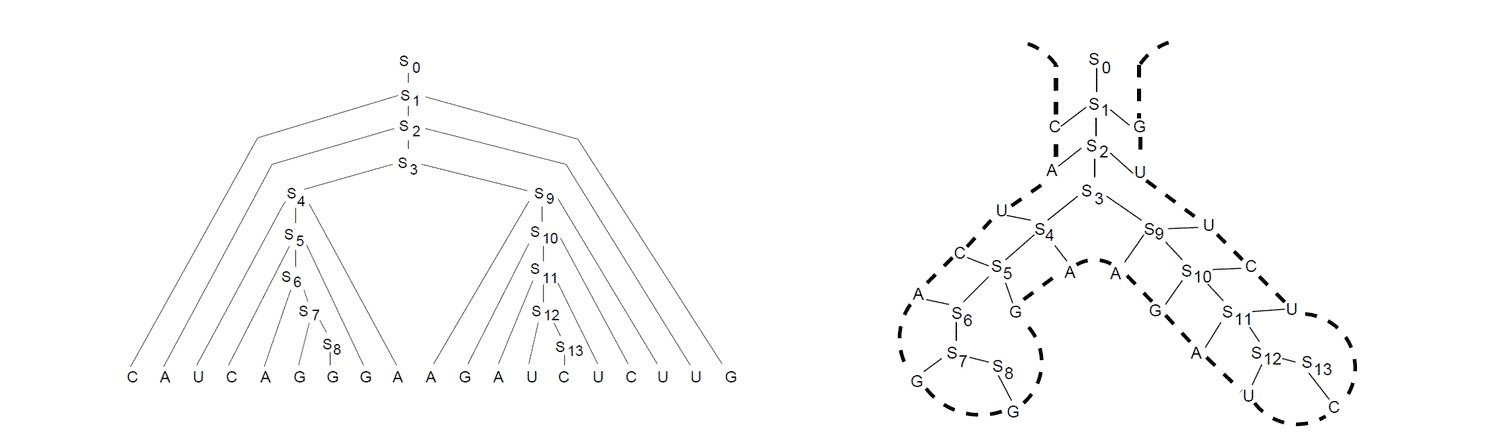
\includegraphics{scfg}}
\end{center}
\caption{Left shows the parse tree for a context free grammar. Right shows how this tree relates to RNA secondary structure. Taken from original publication \cite{sakakibara1994stochastic}.}
\label{fig:scfg}
\end{figure}

\section{The Thermodynamic Hypothesis}
Current state of the art algorithms fold RNA in a way that globally maximises their score according to some model. The Zuker algorithm, for example, finds the global minimum free energy configuration. SCFGs globally maximise the perceived probability of a parse tree. This bias is largely due to the Thermodynamic Hypothesis. Anfinsen \cite{anfinsen1973principles} presented this hypothesis as the underlying principle behind the formation of biologically active proteins. He held that protein fold into the minimum Gibbs free energy conformation in their typical biological environment. (Environment being defined as the molecules' physiological state: pH, temperature, and ion concentration.) Furthermore, through natural selection, molecules that are most likely to fold into the correct shape have evolved. This insight has been invaluable for folding proteins in silico. It has since been applied to the RNA folding problem. Despite this, it has recently become clear that methods for the prediction of RNA secondary structures have hit an upper limit in accuracy.


\section{Conclusions}

The Thermodynamic Hypothesis posits that biologically active molecules will have thermodynamically minimal free energy configurations. I submit that this hypothesis may not entirely hold for RNA molecules. By this I mean that it is insufficiently powerful to explain in vivo RNA secondary structures. As Rivas \cite{rivas2013four} noted, there appears to be a ceiling on the accuracy of our current algorithms. I have given a brief but working summary of these algorithms, stressing their adherence to the Thermodynamic Hypothesis. Perhaps local interactions are stronger factors than global interactions during RNA folding. Alternatively, it could be that the folding pathway itself is more important than the final free energy of the folded molecule. Regardless, finding a way past the accuracy barrier will be important for future advancements, as it is increasingly obvious that RNAs are essential biological agents. If we are to improve our algorithms, then we are in need of a way beyond the Thermodynamic Hypothesis.





%let bibtex do all the hard work
\bibliographystyle{plain}
\bibliography{assignment_two}


\end{document}

